\documentclass{article}
\usepackage{ctex}
\usepackage{amsmath}
\usepackage{graphicx}
\usepackage{wrapfig}
\usepackage{caption}
\usepackage[top=0.8in, bottom=0.8in,left=0.8in, right=0.8in]{geometry}
\usepackage{float} 
\usepackage{subfigure}
\usepackage{subcaption}
\usepackage{bm}
\xeCJKsetup{CJKmath=true} 

\begin{document}
\section*{Kerr盒(40分)}
\begin{wrapfigure}{r}{5cm}
	\vspace{-15pt}    % 对应高度1
	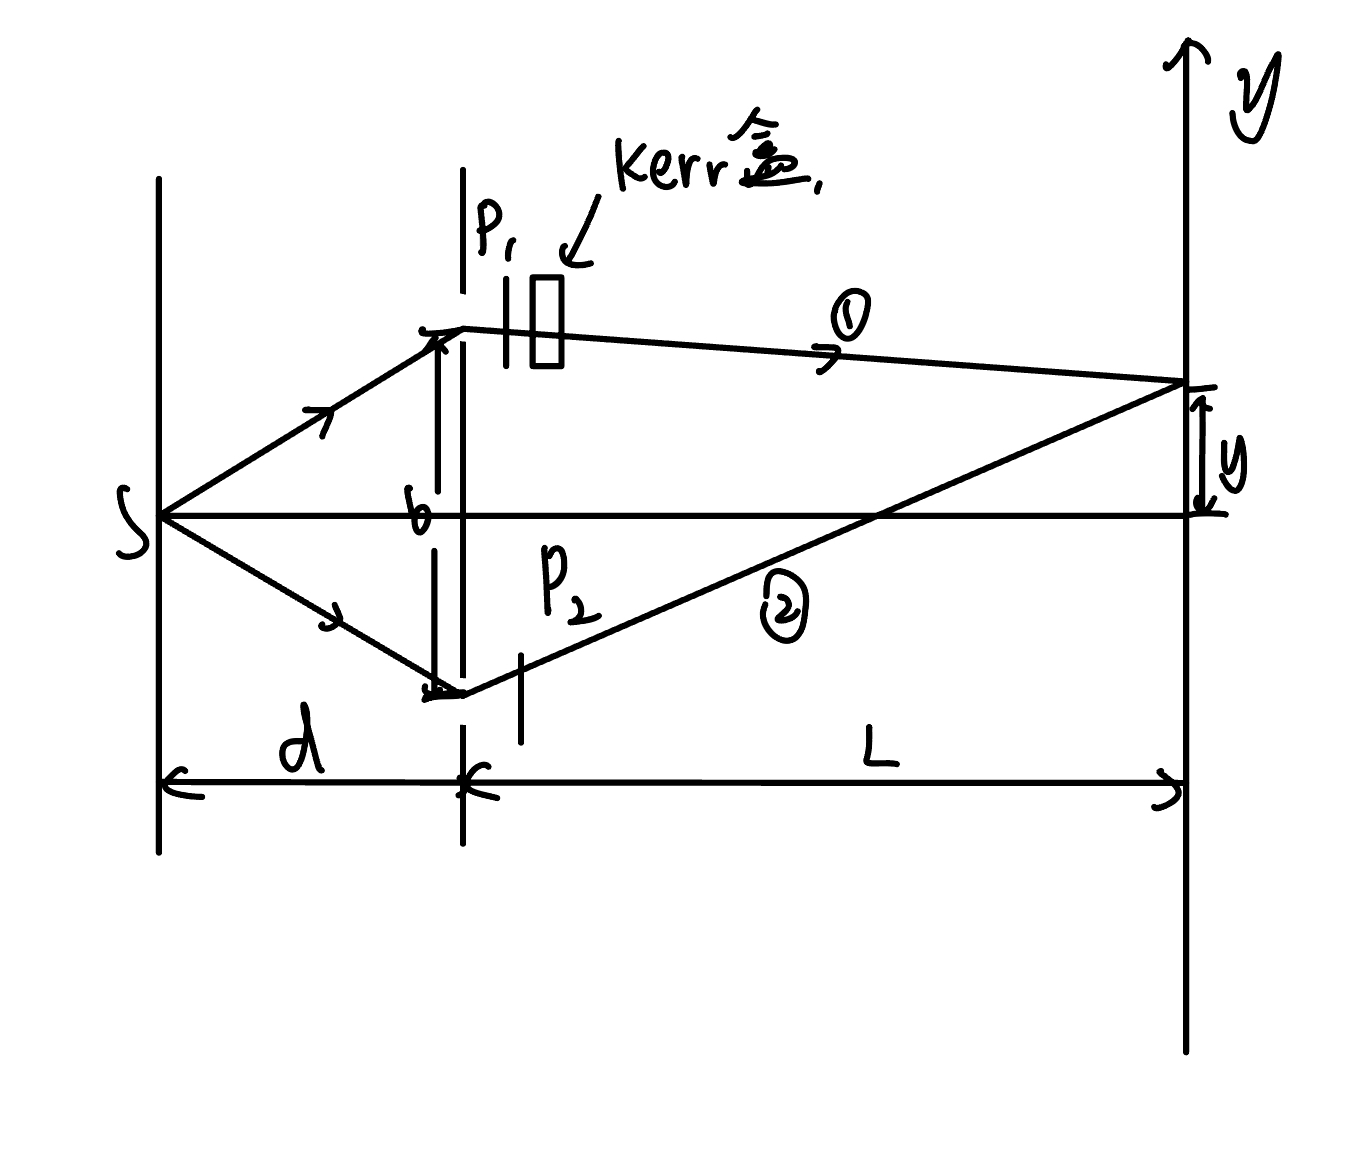
\includegraphics[width=5cm]{img/0013.1.jpeg}\\
	\vspace{-15pt}    % 对应高度2
	\caption{}
	\vspace{-15pt}    % 对应高度3
\end{wrapfigure}
 已知Kerr盒相当于一波晶体片,因其导致o光,e光间光程差满足下式$$\dfrac{\Delta}{2\pi}=\dfrac{|n_o-n_e|d}{2\pi}=B\dfrac{E^2 d}{\lambda}$$其中$d$为Kerr盒长。\par
如图偏针片$P_1, P_2$偏正方向夹角为$\theta$,$o$振动光矢量垂直于主平面.
Kerr盒对应光轴方向垂直于$P_2$偏振方向,双缝干涉参数如图。
\begin{itemize}
    \item[(1)] 试求光线$\textcircled{1}$通过Kerr盒后椭圆偏振光的椭圆参数.即长轴大小,方向(用通过偏振片后振幅$A$表示)
    \item[(2)] 试求屏上光强分布$$T(y)=\dfrac{1}{T}\int^T_0|\vec{E}|^2\mathrm{d} t$$
    \item[(3)] 试求衬比度$$\gamma=\dfrac{I_{max}-I_{min}}{I_{max}+I_{min}}$$
\end{itemize}
\end{document} 